\documentclass[border=10pt]{standalone}
\usepackage{tikz}
\usetikzlibrary{shapes.geometric, arrows.meta, positioning}

\begin{document}
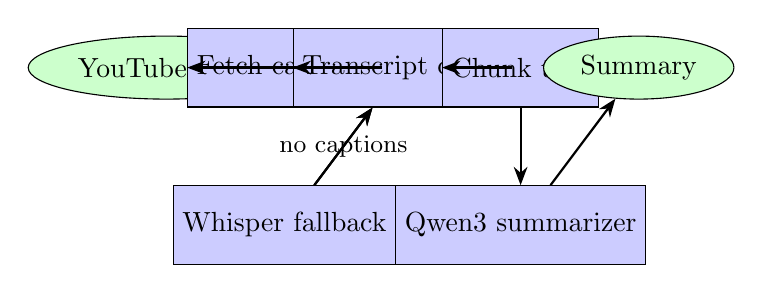
\begin{tikzpicture}[
    node distance=1.5cm,
    ellipse box/.style={ellipse, draw, fill=green!20, minimum width=1.5cm, minimum height=0.8cm},
    rectangle box/.style={rectangle, draw, fill=blue!20, minimum height=1cm, minimum width=1.5cm},
    edge label/.style={font=\small, align=center, xshift=0.5cm, yshift=-0.5cm},
    edge arrow/.style={-Stealth, thick}
]
    % Nodes
    \node[ellipse box] (url) {YouTube URL};
    \node[rectangle box] (fetch) [right of=url] {Fetch captions};
    \node[rectangle box] (cache) [right of=fetch] {Transcript cache};
    \node[rectangle box] (chunk) [right of=cache] {Chunk text};
    \node[ellipse box] (summary) [right of=chunk] {Summary};
    \node[rectangle box] (whisper) [below of=fetch, yshift=-0.5cm] {Whisper fallback};
    \node[rectangle box] (qwen) [below of=chunk, yshift=-0.5cm] {Qwen3 summarizer};

    % Edges
    \draw[edge arrow] (url) -- (fetch);
    \draw[edge arrow] (fetch) -- (cache);
    \draw[edge arrow] (cache) -- (chunk);
    \draw[edge arrow] (chunk) -- (qwen);
    \draw[edge arrow] (qwen) -- (summary);
    \draw[edge arrow] (whisper) -- (cache);
    \draw[edge arrow] (whisper) edge[edge label] node {no captions} (cache);

\end{tikzpicture}
\end{document}
